\documentclass{article}
\usepackage{color}
\usepackage{cite}
\usepackage{hyperref}
\usepackage{graphicx}
\usepackage{siunitx}
\newcommand{\hl}[1]
{\colorbox{yellow}{#1}}
\title{Making Secure Easy-to-Remember Passwords}
\author{Philip Braunstein}
\date{December 14, 2015}
\begin{document}

\maketitle
\abstract{
Password leaks are a notorious way that systems get compromised. Passwords are often leaked exactly because they are heard to remember, which prompts people to record them in insecure locations and avoid changing them. This report describes and evaluates three password generation strategies. Three password generation strategies are evaluated in this report: random strings of characters, numbers, and symbols; abbreviations of phrases mixed with meaningful numbers; and an adjective-noun-verb-adjective-noun string modeled after xkcd 936 \hl{SOURCE: XKCD}. Passwords are evaluated on ease of memorization, cryptographic strength against a password cracker, and bits of entropy
}

\section*{Introduction}
People like to imagine that computer security is usually compromised by genius hackers exploiting inscrutable vulnerabilities. Often however, an attacker compromises a system because of seemingly stupid reasons like the being written on a note next to the computer. Shoring up technical security is a worthy cause, but this effort is rendered irrelevant unless the impact of social engineering resulting in password leaks is minimized. 

People avoid changing their passwords, leave them written in plain text in a document on their computer or even on a sticky note on their computer for one reason only: secure passwords are hard to remember. Insecure and poorly-stored passwords are the cause of many security leaks \hl{FIND SOME GENERAL SOURCES}. Passwords are a common source of vulnerability because different websites have different requirements for what they consider valid passwords, and passwords that are considered secure are obtuse and hard for people to remember.

In this report, three methods for making passwords are described and evaluated. The security and how easy each type of password to remember is evaluated and described in the Results section.

\section*{To the Community}

\section*{Methods}
\subsection*{Overall Description of Procedure}
Each of the password generation methods described below were tested on a total of 7 subjects. In order to prevent bias based on subjects getting used to the memorization task, the script \texttt{determineOrder.py} was used to dictate the order that each of the password methods was tested. For the random string and modified XKCD password style, participants were shown 10 options for passwords and were permitted to chose the preferred password. Participants were told there were no length requirements for the MPM password, and they were not informed of the length of the RS and MX passwords.

For each password method, participants chose the password they wanted to use, and participants were not permitted to write the password down. Participants were then instructed to focus on something else. Most went back to work, and some chatted with me during that time. When I was speaking with a participant, I tried to steer the conversation away from the topic of the password that they chose. After five minutes, participants were asked to write their password down. If they wrote the password down exactly correctly, they were informed that they remembered their password perfectly. If they messed up their password, they were either told what was amiss with their guess (e.g. ``the correct password is \texttt{casualpiebecomesonlyprofit} instead of \texttt{otherpiebecomesonlyprofit} or they were shown the correct password for another couple of seconds. Participants worked or chatted with me for another five minutes, and then wrote down their passwords again. Passwords were tested one at a time. It was at no time during the experiment necessary for participants to remember more than one password. As an example, Participant 1 first only had to remember the random string password, then only the modified XKCD password, and then only the memorable phrase and number password.



\subsection*{Password Generation Schemes}
\subsubsection*{Random String}
A random string password consists of ten random characters, numbers, and symbols. A random string passwords must have contain at least one of three of the four categories: upper-case letter, lower-case letter, number, or symbol. The script \texttt{randomPass.py} generates ten of these random strings passwords. Participants selected one of the ten passwords to use.


\subsubsection*{Memorable Phrase and Number}
Participants chose a memorable phrase and made an acronym of the first letter of each word. Every initial was lower-case in the password. They also chose a particular number and incorporated it after the initials of the memorable phrase. For example, I might choose the hook from a famous Rolling Stones song (\textbf{I} \textbf{c}an't \textbf{g}et \textbf{n}o \textbf{s}atisfaction, and the month and year of my graduation from college (May, 2012) to generate the following password: icgns0512. 

\subsubsection*{Modified XKCD}
Randall Munroe of XKCD suggests using several common words that can be used to create a more coherent memory as opposed to other password generation methods. I have improved on his idea by forcing passwords to obey the form adjective noun verb adjective noun, where the words from these parts of speech are drawn from publicly available word lists \hl{CITE WORD LISTS}.

The script \texttt{humanPass.py} creates ten of these modified XKCD passwords, from which the participant chose one. The passwords were written with all lower case letters and no spaces between the words. Participants were allowed to alter the password to fix any grammatical mistakes. For example one password generated by \texttt{humanPass.py} was \texttt{availablenervebitemolecularradish} (available nerve bite molecular radish). Participants were instructed to modify the passwords so that they make grammatical sense, but the exact modification was left to the discretion of the participant. For example, the previous password could be modified in one of two ways \texttt{availablenervebitesmolecularradish} (available nerve bites molecular radish) or \texttt{availablenervesbitemolecularradish} (available nerves bite molecular radish). Participants were encouraged to make whatever grammatical modification makes the most sense to them.

\subsection*{Password Evaluation}
The passwords were evaluated on three criteria: the success of a participant remembering the password, the strength of the password against password cracking, and the number of bits of entropy.
\subsubsection*{Success Remembering Password}
At first glance, the success of a participant remembering a password should be measured by the percent similarity of the remembered password and the actual password. This could be calculated by comparing each character in the two passwords to see how similar they are. This method, however, is insufficient. Consider the following example:\\


\noindent\texttt{0123456789}\\
\texttt{023456789} \\

These two passwords result in a similarity of 0.1 since the `1' is omitted in the second password. However, nine of ten of the characters were successfully remembered. Therefore, this simple metric of similarity under-represents how similar the two passwords actually are. In short, a simple percent similarity metric does not account for character insertions or deletions in the sequences.

To compensate for this problem, the script \texttt{smartFracSim.py} calculates the fraction similar of the two passwords from the forward direction \emph{and} from the reverse direction and averages these values (hereafter: smart fraction similar). This raises the fraction similar of the example to 0.45 $((0.1 + 0.8 / 2.0))$.

While the smart fraction similar is a better metric than fraction similar of only one direction, I still believed that this metric was under-representing the similarity in the passwords. Consider the modified xkcd example password from above: \\

\noindent \texttt{availablenervebitesmolecularradish} (available nerve bites molecular radish) \\

Consider what would happen if a participant swapped the adjectives to make the following password:\\

\noindent \texttt{molecularnervebitesavailableradish} (molecular nerve bites available radish). \\

The original and adjective-swapped passwords have a smart fraction similar of 0.47. This significantly under-represents the how close the participant was to correctly remembering the password. The participant simply flipped the adjectives, and might score a 1.0 similarity if asked again. In order to compensate for this, the modified XKCD passwords were also analyzed for similarity as follows: what fraction of the original words were also present in the remembered password, regardless of the grammatical form (for example, \texttt{nerve} would count when matched with \texttt{nerves}). This word similarity metric was averaged with the smart fraction similar metric to compute the final similarity for the modified XKCD passwords. In the swapped adjectives example, the word fraction similar is 1.0 (all words are present). Averaged with the smart fraction similar, the final similarity fraction for this example is 0.74. The word fraction was determined by hand (by me), since it would have been difficult to write a script to recognize the varying valid grammatical forms of word as well as where to break the password string into a word.

The word fraction similarity metric is successful because it accounts for distinct parts of the password that a participant has successfully remembered. There is no exact corresponding metric for the random string and memorable phrase and number passwords. So, the fraction of characters similar between the original password and remembered password was determined for these styles of password using the script \texttt{charFracSim.py}. As above, this metric is averaged with the smart fraction similar to calculate the final similarity for random string and memorable phrase and number passwords.


\subsubsection*{Strength Against Password Cracking}
The MD5 hash of the passwords was determined using built in Python hashing functionality with the script \texttt{makeHashes.py}. A distribution of Kali Linux running in a virtual machine on my Mac was used for the password cracking. 2 GB of RAM was allocated to the virtual machine. The mask attack of the program Hashcat was used for cracking the RS and the MPM passwords. The mask attack is a brute-force attack in which the user supplies a mask which describes the type of characters that should be attempted at each position where \%d signifies a digit, \%l signifies a lower-case letter, and \%a signifies all possible characters. The mask makes the brute-force attack more efficient and more targeted.

The complete invocation of Hashcat to attempt to break RS password hashes was: \\

\texttt{time /usr/bin/hashcat --hash 0 --attack-mode 3 --pw-min 10 hashes.txt \%a\%a\%a\%a\%a\%a\%a\%a\%a\%a} \\

where \texttt{--hash 0} indicates that MD5 without salt was used to has the passwords, \texttt{--attack-mode 3} indicates a mask attack should be used, \texttt{--pw-min} indicates the smallest length password guessed should be 10 (so Hashcat didn't increment through shorter length password guesses), \texttt{hashes.txt} is the file containing the hashes, and \texttt{\%a\%a\%a\%a\%a\%a\%a\%a\%a\%a} is the mask that indicates each of the 10 positions could be any character (equivalent to the deprecated brute-force attack). 

The MPM passwords have the predictable structure of a number of lower case letters followed by a couple of digits. Several runs of Hashcat with masks corresponding to the structure of every MPM password created by the participants of this study. The masks used were \texttt{\%l\%l\%l\%l\%d\%d}, \texttt{\%l\%l\%l\%l\%d\%d\%d\%d}, \texttt{\%l\%l\%l\%l\%l\%d\%d}, and \texttt{\%l\%l\%l\%l\%l\%d\%d\%d\%d}. The standard Unix function \texttt{time} was used to record the user time it took to run each cracking attempt.

Password cracking was not attempted to crack the hashes of the MX passwords because these passwords are far too long to be cracked with a mask attack. Calculations to approximate resistance to hacking attacks of the MX passwords is described in the results section.

\subsubsection*{Bits of Entropy}
The bits of entropy for each password was determined by calculating the number of possible passwords for a password of that style of that length. The entropy of the RS passwords ($H_{RS}$) was determined by the following formula:

$$H_{RS} = 94^{10}$$

in which there were 94 possibilities for each character and the overall length of the password was 10 characters. The 94 possibilities came from the following Python statement: \\

\texttt{len(strings.punctuation + strings.digits + strings.letters)}

The entropy of a MPM password $p$ ($H_{MPM}(p)$)was determined as follows:

$$H_{MPM}(p) = 26^l10^d$$

where $l$ is the number of lowercase letters in the MPM password and $d$ is the number of digits in the password.

The entropy of a MX password $p$ ($H_{MX}(p)$) was determined as follows:

$$H_{MX}(p) = 26^{len(p)}$$

MX passwords only contained lowercase letters, which is the derivation of the 26 possibilities per character.


\section*{Results}
\begin{figure}[h]
\centering
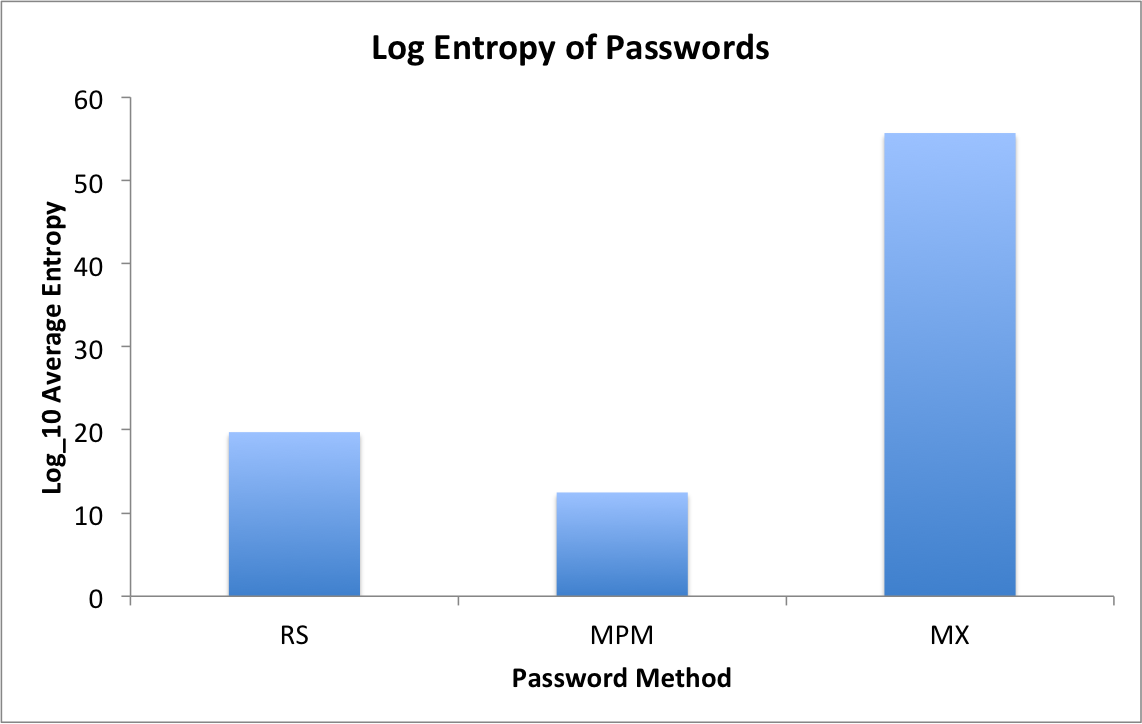
\includegraphics[scale=0.7]{entropy.png}
\caption{Log 10 average entropy of passwords by generation method}
\end{figure}

\begin{table}[h]
\centering
\begin{tabular}{|c|c|c|}
\hline
Password type & Entropy & $log_{10}$ Entropy \\
\hline
RS & \num{5.4e19}& 19\\
\hline
MPM & \num{4.6e11}& 11\\
\hline
MX & \num{5.7e55}& 56\\
\hline
\end{tabular}
\caption{Average Entropy by password generation method}
\end{table}

\begin{table}[h]
\centering
\begin{tabular}{|c|c|c|c|}
\hline
& RS & MPM & MX \\
\hline
RS & 1 & \num{8.6e-9} & \num{1.1e36} \\
\hline
MPM & \num{1.2e8} & 1 & \num{1.2e44}\\
\hline
MX & \num{9.5e-37}& \num{8.2e-45}& 1 \\
\hline
\end{tabular}
\caption{Entry $(x,y)$ is $\frac{\bar{H_x}}{\bar{H_y}}$ where $\bar{H}$ is average entropy}
\end{table}

\begin{figure}
\centering
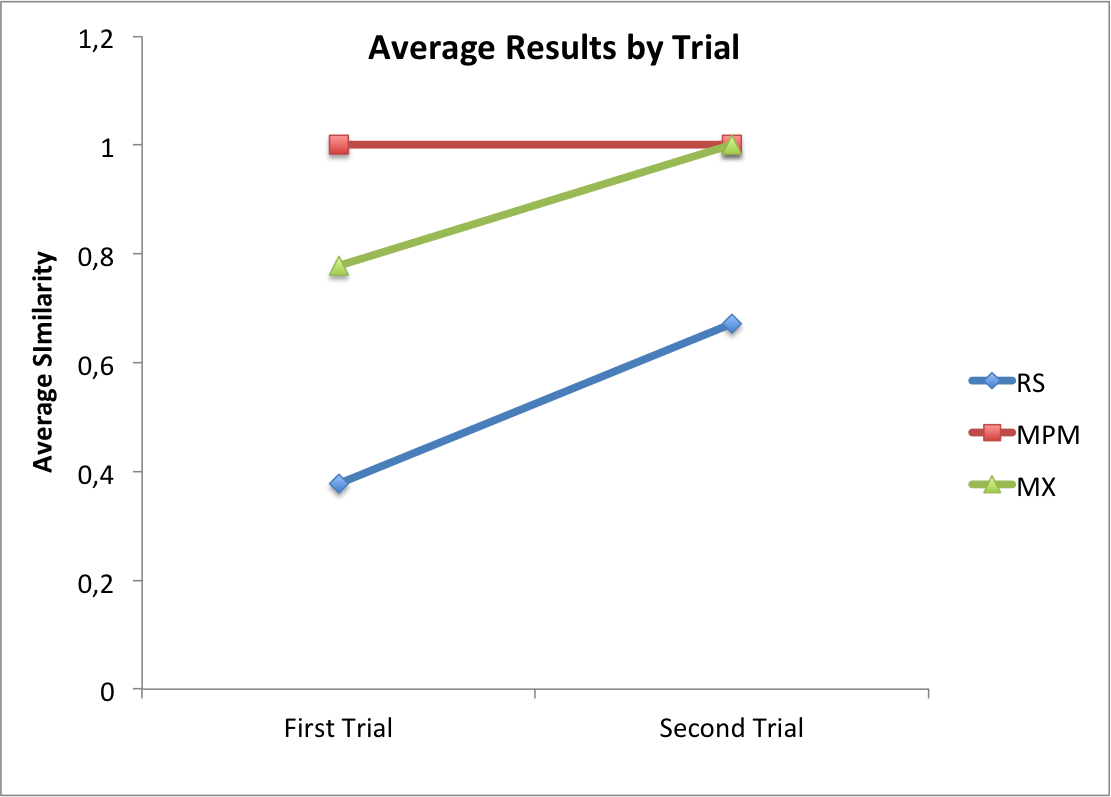
\includegraphics[scale=0.75]{resultsByTrial.png}
\caption{Average similarity by trial and password type}
\end{figure}


\section*{Applications}

\section*{Conclusion}


\end{document}